% AI6103 team report: reimplementation of CIDA (Kundu et al., ECCV 2020).
% Format: CVPR author kit (https://github.com/cvpr-org/author-kit, release CVPR2027-v1).
% Sections are in sec/, figures in fig/. Section 4 (Experiments) is written by the team.
% Placeholders use \TODO{...} (defined in preamble.tex). Remove them all before submission.

\documentclass[10pt,twocolumn,letterpaper]{article}

%%%%%%%%% PAPER TYPE
% Camera-ready layout (author names shown, no review line numbers) with page numbers.
\usepackage[pagenumbers]{cvpr}

% Import additional packages in the preamble file, before hyperref
%% This file contains a number of tweaks that are typically applied to the main document.
%% They are not enabled by default, but can be enabled by uncommenting the relevant lines.


%%
%% Inline annotations; for predefined colors, refer to "dvipsnames" in the xcolor package:
%% https://tinyurl.com/overleaf-colors
%%
\newcommand{\red}[1]{{\color{red}#1}}
\newcommand{\todo}[1]{{\color{red}#1}}
\newcommand{\TODO}[1]{\textbf{\color{red}[TODO: #1]}}
%%
%% Disable for camera ready / submission by uncommenting these lines:
%%
% \renewcommand{\TODO}[1]{}
% \renewcommand{\todo}[1]{#1}

%%
%% Work harder in optimizing text layout. Typically shrinks text by 1/6 of page, enable
%% it at the very end of the writing process, when you are just above the page limit.
%%
% \usepackage{microtype}

%%
%% Fine-tune paragraph spacing.
%%
% \renewcommand{\paragraph}[1]{\vspace{.5em}\noindent\textbf{#1.}}

%%
%% Globally adjusts space between figure and caption.
%%
% \setlength{\abovecaptionskip}{.5em}

%%
%% Allows "the use of \paper to refer to the project name"
%% with automatic management of space at the end of the word.
%%
% \usepackage{xspace}
% \newcommand{\paper}{ProjectName\xspace}

%%
%% Commonly used math definitions.
%%
% \DeclareMathOperator*{\argmin}{arg\,min}
% \DeclareMathOperator*{\argmax}{arg\,max}

%%
%% Tighten underline.
%%
% \usepackage{soul}
% \setuldepth{foobar}

%%
%% Reconfigure paragraph (tweaks spacing)
%%


%%
%% ----------------------------------------------------------------------------
%% Additions for the CIDA report (the tweaks above came with the original CVPR kit preamble).
%% aaai2027.sty loads the fonts (newtxtext, helvet, courier), T1 encoding and xcolor, and main.tex
%% loads graphicx, natbib, caption and booktabs, so they are not repeated here.
%% Do not add hyperref or any other package that AAAI forbids (see the kit's CameraReady2027.tex).
%% ----------------------------------------------------------------------------
%%
\usepackage{amsmath}
\usepackage{amssymb}
\usepackage{bm}         %< bold math symbols
\usepackage{tabularx}   %< Table 2
\usepackage{tikz}       %< Figure 1 (fig/arch.tex)
\usetikzlibrary{positioning,arrows.meta,calc,fit,backgrounds,shapes.geometric}
\usepackage[capitalize]{cleveref}  %< \cref; works without hyperref
\crefname{section}{Sec.}{Secs.}
\Crefname{section}{Section}{Sections}
\Crefname{table}{Table}{Tables}
\crefname{table}{Tab.}{Tabs.}

%% Notation
\newcommand{\Cs}{\mathcal{C}_s}
\newcommand{\Ct}{\mathcal{C}_t}
\newcommand{\Cp}{\mathcal{C}'_t}
\newcommand{\U}{\mathcal{U}}
\newcommand{\V}{\mathcal{V}}
\newcommand{\Ps}{\mathcal{P}_s}
\newcommand{\Pt}{\mathcal{P}_t}
\newcommand{\Bt}{\mathcal{B}_t}
\newcommand{\Ds}{\mathcal{D}_s}
\newcommand{\Dt}{\mathcal{D}_t}
\newcommand{\lce}{\ell_{\mathrm{ce}}}
\newcommand{\E}{\mathbb{E}}
\newcommand{\vg}{\mathbf{v}_g}
\newcommand{\x}{\mathbf{x}}
\newcommand{\uu}{\mathbf{u}}
\newcommand{\fv}{\mathbf{v}}
\newcommand{\unk}{\varnothing}


\definecolor{cvprblue}{rgb}{0.21,0.49,0.74}
\usepackage[pagebackref,breaklinks,colorlinks,allcolors=cvprblue]{hyperref}

\def\confName{CVPR}
\def\confYear{2027}

%%%%%%%%% TITLE
\title{Reimplementing Class-Incremental Domain Adaptation}

%%%%%%%%% AUTHORS
\author{\TODO{Team member names and matriculation numbers}\\
AI6103 Deep Learning and Applications\\
Nanyang Technological University
}

\begin{document}
\maketitle
\begin{abstract}
Class-Incremental Domain Adaptation (CIDA)~\citep{kundu2020cida} adapts a trained classifier to a new domain that also contains new classes.
It works without the source data and needs only one labelled image per new class.
Since the paper has no public code, we reimplement CIDA from scratch in PyTorch and first run it exactly as the paper describes it.
This version falls well short of the reported accuracy, and we trace the gap to four causes that each call for one change.
The changes re-estimate BatchNorm statistics on the target and start the domain projections at the exact identity.
They also train one pseudo-label loss on confident samples only and freeze the ImageNet backbone.
With these changes, \TODO{headline results, e.g.\ ALL and PRIV on Digits M$\to$U and Office-31, against the paper}.
We also show that the paper's $3\sigma$ rule for negative samples accepts almost every candidate in high dimensions.
\end{abstract}

\section{Introduction}\label{sec:intro}

A deployed classifier often meets data that differ from its training data, and two kinds of change can happen at once.
The images may look different, which is known as \emph{domain shift}.
The new domain may also contain classes the model has never seen, which we call \emph{target-private classes}.
For example, an object recogniser trained on city scenes may be deployed in rural areas, where both the scenes and the objects differ~\citep{kundu2020cida}.

Existing methods handle only one of these changes.
Unsupervised domain adaptation (DA) aligns the two domains, but it assumes that both share one label set~\citep{ganin2016dann}.
Open-set and universal DA methods do detect new classes, but they merge all of them into a single ``unknown'' class~\citep{saito2018osbp,liu2019sta,you2019uan}.
Class-incremental (CI) learning adds new classes over time, yet it ignores domain shift and usually needs labelled data or the source data~\citep{li2017lwf,rebuffi2017icarl,castro2018e2e,dhar2019lwm}.

Kundu et~al.~\citep{kundu2020cida} define the CIDA setting to cover both changes under three constraints.
The first is that the source data are not available during adaptation, which makes the method \emph{source-free}.
The second is that the target images are unlabelled.
The third is that each target-private class has exactly one labelled image, which the paper calls the \emph{one-shot} setting.
Under these constraints, the goal is to classify both the shared and the new classes in the target domain.

Their method works in two stages.
The first stage trains the source model so that each class forms a compact Gaussian cluster in feature space.
It also trains the classifier on synthetic negative samples, which reserves room for classes the model has not yet seen.
The second stage adapts the model in a new feature space for the target, where learnable class centres called \emph{guides} provide the pseudo-labels.

We chose this paper under Option~1 of the assignment, which asks for the reimplementation of a paper without public code.
CIDA was published at ECCV 2020, and its authors did not release their code.
Our work makes four contributions.
\begin{itemize}
  \item \textbf{An implementation from scratch.} It has approximately 940 lines of Python for the method and 410 for analysis tools, not counting blank and comment lines. It also comes with 23 tests and job scripts for a SLURM cluster.
  \item \textbf{A reproduction of the method as written.} A configuration preset switches off all of our changes, so we can run the method exactly as the paper describes it. We use this reproduction to locate where accuracy is lost.
  \item \textbf{Four changes to the method.} Each change addresses one cause of the accuracy loss (\cref{sec:changes}).
  \item \textbf{Checks on unclear parts of the paper.} We list the settings the paper leaves open and three inconsistencies in it. The most important is a $3\sigma$ rule for negative samples that fails in high dimensions (\cref{sec:inconsistencies}).
\end{itemize}

\section{Method}\label{sec:method}

This section describes CIDA as the paper and its supplementary material specify it~\citep{kundu2020cida}.
\Cref{sec:implementation} then lists the details we had to choose ourselves and the changes we made.

% Figure 1: CIDA architecture (simplified from docs/cida_architecture.drawio).
\begin{figure*}[t]
\centering
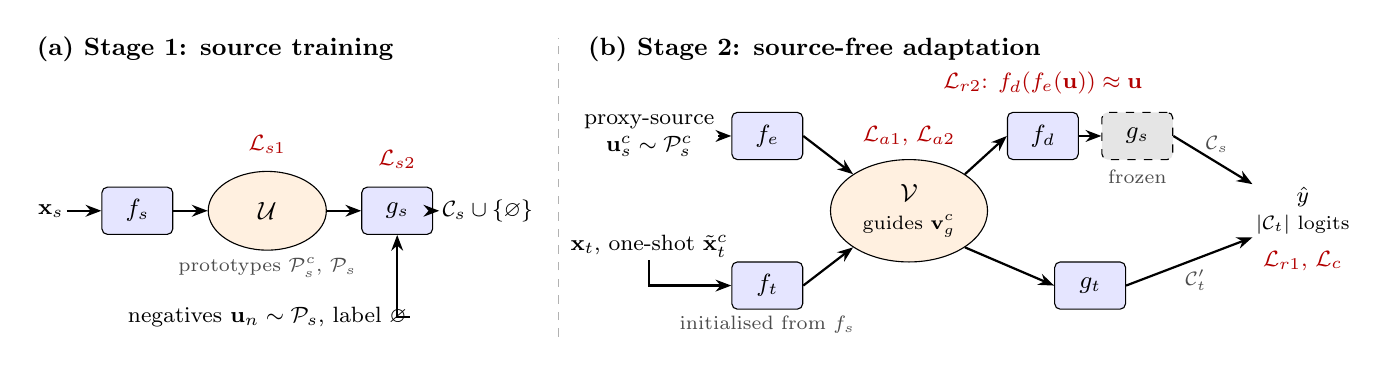
\begin{tikzpicture}[
  font=\small,
  >={Stealth[length=2mm]},
  net/.style={draw, rounded corners=2pt, minimum width=9mm, minimum height=6mm, fill=blue!10},
  frz/.style={draw, dashed, rounded corners=2pt, minimum width=9mm, minimum height=6mm, fill=gray!20},
  sp/.style={draw, ellipse, minimum width=15mm, minimum height=10mm, fill=orange!12},
  io/.style={inner sep=1pt, font=\footnotesize, align=center},
  loss/.style={font=\footnotesize, text=red!70!black},
  note/.style={font=\scriptsize, text=black!70},
  ttl/.style={font=\small\bfseries, anchor=west},
  ar/.style={->, thick},
]
% ---------------------------------------------------------------- (a) Stage 1
\node[ttl] at (-0.3,2.05) {(a) Stage 1: source training};
\node[io] (xs) at (0,0) {$\x_s$};
\node[net] (fs) at (1.1,0) {$f_s$};
\node[sp] (U) at (2.75,0) {$\U$};
\node[note] at (2.75,-0.72) {prototypes $\Ps^c$, $\Ps$};
\node[net] (gs) at (4.4,0) {$g_s$};
\node[io] (os) at (5.55,0) {$\Cs\cup\{\unk\}$};
\node[io] (neg) at (2.75,-1.35) {negatives $\uu_n\sim\Ps$, label $\unk$};
\draw[ar] (xs) -- (fs);
\draw[ar] (fs) -- (U);
\draw[ar] (U) -- (gs);
\draw[ar] (gs) -- (os);
\draw[ar] (neg.east) -| (gs.south);
\node[loss, above=1mm of U] {$\mathcal{L}_{s1}$};
\node[loss, above=1mm of gs] {$\mathcal{L}_{s2}$};

% divider
\draw[black!30, dashed] (6.45,-1.6) -- (6.45,2.2);

% ---------------------------------------------------------------- (b) Stage 2
\begin{scope}[xshift=7.6cm]
\node[ttl] at (-0.9,2.05) {(b) Stage 2: source-free adaptation};
\node[io] (px) at (0,0.95) {proxy-source\\$\uu_s^c\sim\Ps^c$};
\node[net] (fe) at (1.5,0.95) {$f_e$};
\node[io] (xt) at (0,-0.45) {$\x_t$, one-shot $\tilde{\x}_t^c$};
\node[net] (ft) at (1.5,-0.95) {$f_t$};
\node[note] at (1.5,-1.45) {initialised from $f_s$};
\node[sp, minimum width=17mm, minimum height=13mm, align=center] (V) at (3.3,0.0) {$\V$\\[-1pt]{\scriptsize guides $\vg^c$}};
\node[net] (fd) at (5.0,0.95) {$f_d$};
\node[frz] (gs2) at (6.2,0.95) {$g_s$};
\node[note] at (6.2,0.43) {frozen};
\node[net] (gt) at (5.6,-0.95) {$g_t$};
\node[io] (yh) at (8.3,0.0) {$\hat{y}$\\{\scriptsize $|\Ct|$ logits}};
\draw[ar] (px) -- (fe);
\draw[ar] (fe.east) -- (V.north west);
\draw[ar] (xt.south) |- (ft.west);
\draw[ar] (ft.east) -- (V.south west);
\draw[ar] (V.north east) -- (fd.west);
\draw[ar] (fd) -- (gs2);
\draw[ar] (V.south east) -- (gt.west);
\draw[ar] (gs2.east) -- node[above, note, pos=0.55] {$\Cs$} (yh.north west);
\draw[ar] (gt.east) -- node[below, note, pos=0.55] {$\Cp$} (yh.south west);
\node[loss, above=1mm of fd] {$\mathcal{L}_{r2}$: $f_d(f_e(\uu))\approx\uu$};
\node[loss, above=0.5mm of V] {$\mathcal{L}_{a1}$, $\mathcal{L}_{a2}$};
\node[loss, below=0.5mm of yh] {$\mathcal{L}_{r1}$, $\mathcal{L}_{c}$};
\end{scope}
\end{tikzpicture}
\caption{CIDA architecture. The source data never enter Stage~2, where Gaussian prototypes replace them.
(a)~Stage~1 trains $f_s$ and $g_s$. $\mathcal{L}_{s1}$ makes each class a compact cluster around its prototype, and $\mathcal{L}_{s2}$ teaches $g_s$ to assign synthetic negatives to the extra class $\unk$.
(b)~Stage~2 trains a target extractor $f_t$, a classifier $g_t$ for the new classes and two projections $f_e$ and $f_d$ between $\U$ and $\V$, while $g_s$ stays frozen.
Red labels show where each loss is computed, and \cref{tab:losses} lists the networks each loss updates.}
\label{fig:arch}
\end{figure*}


\subsection{Problem setting}\label{sec:setting}
The labelled source set is $\Ds=\{(\x_s,y_s)\}$ with label set $\Cs$.
The unlabelled target set $\Dt=\{\x_t\}$ is drawn from the marginal distribution $q_X$ and has a larger label set $\Ct\supset\Cs$.
The target-private classes are $\Cp=\Ct\setminus\Cs$, and each class $c\in\Cp$ comes with one labelled target image $\tilde{\x}_t^c$.
The source data are not available during adaptation.

\subsection{Stage 1: source training}\label{sec:stage1}
A feature extractor $f_s$ maps images to a feature space $\U$, and a classifier $g_s$ maps these features to $|\Cs|+1$ outputs.
The extra output, denoted $\unk$, stands for ``none of the source classes''.

\paragraph{Gaussian prototypes.}
For each class $c\in\Cs$, a Gaussian $\Ps^c=\mathcal{N}(\bm{\mu}_s^c,\bm{\Sigma}_s^c)$ is fitted to the features $f_s(\x_s)$ of that class.
A global Gaussian $\Ps=\mathcal{N}(\bm{\mu}_s,\bm{\Sigma}_s)$ is fitted to all source features in the same way.
These prototypes are all that Stage~2 keeps of the source data.

\paragraph{Class separability ($\mathcal{L}_{s1}$).}
This loss is a cross-entropy in which the class prototypes act as the classifier.
With $\uu_s=f_s(\x_s)$, it reads
\begin{equation}
  \mathcal{L}_{s1} = \E_{(\x_s,y_s)}\Big[-\log\frac{\exp \ell^{y_s}(\uu_s)}{\sum_{c\in\Cs}\exp \ell^{c}(\uu_s)}\Big],
  \label{eq:ls1}
\end{equation}
where $\ell^c(\uu)$ scores $\uu$ under $\Ps^c$.
The paper uses the density $\Ps^c(\uu)$ as this score, while we use the log-density $\log\Ps^c(\uu)$ for numerical reasons (\cref{sec:choices}).
Minimising the loss makes each class a compact cluster around its prototype.

\paragraph{Negative samples ($\mathcal{L}_{s2}$).}
Negative features $\uu_n$ represent regions of $\U$ where the source density is low.
To create one, we draw a candidate $\uu\sim\Ps$ from the global Gaussian and find its most likely class $\hat c=\arg\max_c \Ps^c(\uu)$.
Let $\lambda$ be the largest eigenvalue of $\bm{\Sigma}_s^{\hat c}$ and $\bm{\nu}$ its eigenvector.
The candidate is kept as a negative if
\begin{equation}
  \Ps^{\hat c}(\uu) < \Ps^{\hat c}\big(\bm{\mu}_s^{\hat c}+3\sqrt{\lambda}\,\bm{\nu}\big),
  \label{eq:neg}
\end{equation}
that is, if it lies outside the $3\sigma$ region of class $\hat c$.
The classifier then learns to assign these negatives to $\unk$ through
\begin{equation}
  \mathcal{L}_{s2} = \E_{(\x_s,y_s)}\,\lce\big(g_s(f_s(\x_s)),y_s\big) + \E_{\uu_n}\,\lce\big(g_s(\uu_n),\unk\big),
  \label{eq:ls2}
\end{equation}
where each batch holds as many negatives as source images.

\paragraph{Optimisation.}
One warm-up epoch first trains $f_s$ and $g_s$ with plain cross-entropy, which gives the first prototypes.
Training then alternates between the two losses, one per iteration.
$\mathcal{L}_{s1}$ updates only $f_s$, while $\mathcal{L}_{s2}$ updates both $f_s$ and $g_s$.
Each loss has its own Adam optimiser~\citep{kingma2015adam} with learning rate $10^{-4}$, and the prototypes are refitted after every epoch.
The final source model consists of $f_s$, $g_s$ and the prototypes $\{\Ps^c\}$ and $\Ps$.

\subsection{Stage 2: adaptation to the target}\label{sec:stage2}

\paragraph{Networks.}
The target feature extractor $f_t$ is initialised from $f_s$ and maps images to a new space $\V$.
A new classifier $g_t$ has one output per class in $\Cp$, while the source classifier $g_s$ stays frozen.
Two domain projections, $f_e:\U\to\V$ and $f_d:\V\to\U$, connect the two feature spaces.
Stage~2 replaces the source data with \emph{proxy-source} samples, which are features drawn from the prototypes, $\uu\sim\Ps^c$.
Before adaptation, $f_e$ and $f_d$ are pretrained towards the identity by minimising $\|f_e(\uu)-\uu\|^2$ and $\|f_d(\uu)-\uu\|^2$ on these samples.
For a feature $\fv\in\V$, the model then outputs $|\Ct|$ logits,
\begin{equation}
  \hat{y}(\fv) = \big[\,g_s(f_d(\fv))\big|_{\Cs}\;;\; g_t(\fv)\,\big],
  \label{eq:yhat}
\end{equation}
where the first part keeps the $|\Cs|$ shared-class logits of $g_s$ and drops $\unk$.

\paragraph{Retaining the source classes ($\mathcal{L}_{r1}$, $\mathcal{L}_{r2}$).}
Proxy-source samples $\uu_s^c\sim\Ps^c$ with $c\in\Cs$ enter two losses that preserve the source classes,
\begin{align}
  \mathcal{L}_{r1} &= \E_{c,\,\uu_s^c}\,\lce\big(\hat{y}(f_e(\uu_s^c)),c\big),\label{eq:lr1}\\
  \mathcal{L}_{r2} &= \E_{c,\,\uu_s^c}\,\big\|f_d(f_e(\uu_s^c))-\uu_s^c\big\|^2.\label{eq:lr2}
\end{align}
$\mathcal{L}_{r1}$ keeps the source classes recognisable after the round trip through $f_e$ and $f_d$.
$\mathcal{L}_{r2}$ keeps $f_d$ an inverse of $f_e$, which stops the projections from discarding information.

\paragraph{Guides and pseudo-labels.}
Each class $c\in\Ct$ has a guide $\vg^c\in\V$, which acts as its class centre in the target space,
\begin{equation}
  \vg^c = f_e(\bm{\mu}_s^c)\ \ \text{for } c\in\Cs,
  \qquad
  \vg^c = f_t(\tilde{\x}_t^c)\ \ \text{for } c\in\Cp.
  \label{eq:guides}
\end{equation}
The shared guides can move during adaptation, because $f_e$ is trained.
Each target sample receives the label of its nearest guide, $k(\x_t)=\arg\min_{c}\|f_t(\x_t)-\vg^c\|_2$.
Gaussian prototypes $\Pt^c$ are then fitted to the pseudo-labelled target features.
The confident set $\Bt^c$ holds the $n=20\%$ of samples labelled $c$ that lie closest to $\vg^c$.
The pseudo-labels, $\Pt^c$ and $\Bt^c$ are all recomputed after every epoch.

\paragraph{Alignment ($\mathcal{L}_{a1}$, $\mathcal{L}_{a2}$) and classification ($\mathcal{L}_{c}$).}
With $\fv_t=f_t(\x_t)$, the remaining three losses are
\begin{align}
  \mathcal{L}_{a1} &= \E_{\x_t\sim q_X}\Big[-\log\frac{\exp\ell_t^{k(\x_t)}(\fv_t)}{\sum_{c\in\Ct}\exp\ell_t^{c}(\fv_t)}\Big],\label{eq:la1}\\
  \mathcal{L}_{a2} &= \E_{c,\,\x_t\in\Bt^c}\,\|\fv_t-\vg^c\|^2,\label{eq:la2}\\
  \mathcal{L}_{c}  &= \E_{c,\,\x_t\in\Bt^c}\,\lce\big(\hat{y}(\fv_t),c\big),\label{eq:lc}
\end{align}
where $\ell_t^c$ is the score under $\Pt^c$.
$\mathcal{L}_{a1}$ separates the target clusters and makes room for the new classes.
$\mathcal{L}_{a2}$ pulls confident samples towards their guides, and $\mathcal{L}_{c}$ trains the classifiers on the confident pseudo-labels.

\paragraph{Optimisation.}
Each loss has its own Adam optimiser and updates only some of the networks, as \cref{tab:losses} shows.
The losses take turns in a fixed cycle, with one loss per iteration.
Because separate optimisers scale the gradients of each loss independently, the paper needs no loss weights.

\begin{table}[t]
  \centering
  \small
  \caption{Stage~2 losses and the networks each one updates. The source classifier $g_s$ stays frozen throughout.}
  \label{tab:losses}
  \begin{tabular}{@{}lll@{}}
    \toprule
    Loss & Samples & Updates \\
    \midrule
    $\mathcal{L}_{r1}$ \eqref{eq:lr1} & proxy-source $\uu_s^c\sim\Ps^c$ & $f_e, f_d, g_t$ \\
    $\mathcal{L}_{r2}$ \eqref{eq:lr2} & proxy-source $\uu_s^c\sim\Ps^c$ & $f_e, f_d$ \\
    $\mathcal{L}_{c}$ \eqref{eq:lc}   & confident set $\Bt$              & $f_t, g_t$ \\
    $\mathcal{L}_{a1}$ \eqref{eq:la1} & all target samples               & $f_t$ \\
    $\mathcal{L}_{a2}$ \eqref{eq:la2} & confident set $\Bt$              & $f_e, f_t$ \\
    \bottomrule
  \end{tabular}
\end{table}

\paragraph{Prediction.}
The predicted class of a target image $\x$ is $\arg\max_{c\in\Ct}\hat{y}(f_t(\x))_c$.
In the paper's few-shot setting, with several labelled images per private class, each private guide is the mean feature of those images.

\section{Implementation}\label{sec:implementation}

We implemented the method in PyTorch without any reference code.
Each stage is one script, and a separate module handles prototype fitting, log-densities and sampling.

\paragraph{Networks.}
We follow the architectures in the paper's supplementary material.
For Digits, $f_s$ is a modified LeNet with BatchNorm and 100-dimensional features.
For Office-31 and VisDA, $f_s$ is an ImageNet-pretrained ResNet-50~\citep{he2016resnet}.
A head of three fully connected layers (1024, 256 and 256 units) with ELU activations and BatchNorm follows it and produces 256-dimensional features.
The classifiers $g_s$ and $g_t$ are two-layer MLPs.
The projections $f_e$ and $f_d$ have two fully connected layers for Digits and three for Office and VisDA.

\subsection{Choices the paper leaves open}\label{sec:choices}
\Cref{tab:choices} lists the settings the paper does not give, together with our choices.
We tuned the Digits epoch counts on M$\to$U only and then kept them fixed for the other Digits tasks.

\begin{table}[t]
  \centering
  \small
  \caption{Settings not specified in the paper, and our choices.}
  \label{tab:choices}
  \begin{tabularx}{\columnwidth}{@{}>{\raggedright\arraybackslash}p{2.0cm}>{\raggedright\arraybackslash}X@{}}
    \toprule
    Setting & Our choice and reason \\
    \midrule
    Prototype score $\ell^c$ & $\log\mathcal{P}^c(\uu)$, because raw densities in 100 to 256 dimensions underflow. \\
    Covariance & $\bm{\Sigma}\leftarrow 0.9\,\bm{\Sigma} + (0.1+10^{-4})\,\tfrac{\operatorname{tr}\bm{\Sigma}}{D}\,\mathbf{I}$. An Office class has approximately 30 to 90 images in 256 dimensions, so its raw covariance is singular. \\
    Batch size & 64 for Digits, 32 for Office and VisDA. \\
    Source epochs & 10 (Digits), 50 (Office), 5 (VisDA). \\
    Adaptation epochs & 30 (Digits), 60 (Office), 10 (VisDA). \\
    Adaptation epoch length & Five times the number of target batches, so each of the five losses sees approximately one pass over the target data. \\
    Projection pretraining & 2{,}000 iterations. \\
    Data splits & Digits adapts on the target training split and tests on the target test split. Office adapts and tests on the whole target domain, minus the labelled images. \\
    Warm-up & Updates both $f_s$ and $g_s$. The algorithm lists only $f_s$, but $g_s$ also needs training. \\
    Private guides & One-shot images pass through $f_t$ in the same batch as target samples, so BatchNorm never sees a batch of only one image per class. \\
    \bottomrule
  \end{tabularx}
\end{table}

\subsection{Our changes to the method}\label{sec:changes}
When we ran the method as written, shared and private classes became mixed during adaptation (\cref{sec:exp-vanilla}).
We made four changes, each aimed at one cause, and \cref{sec:exp-improvements} reports their effect.
A configuration preset (\texttt{preset=vanilla}) switches all four off.

\paragraph{1. Target BatchNorm statistics.}
Because $f_t$ starts as a copy of $f_s$, it also inherits the BatchNorm running statistics of the source domain.
The first pseudo-labels are computed with these statistics, which creates a mismatch.
The private guides come from target images, while the shared guides come from source means.
As a result, many shared target samples lie closer to a private guide than to their own shared guide.
Before adaptation, we therefore re-estimate the BatchNorm statistics of $f_t$ on the unlabelled target set, a technique known as AdaBN~\citep{li2018adabn}.
This fits the design of the method, since $f_t$ is meant to be specific to the target.

\paragraph{2. Projections that start as the exact identity.}
The paper pretrains $f_e$ and $f_d$ as plain MLPs to approximate the identity, but some error remains after pretraining.
This error moves shared-class features across the decision boundaries of $g_s$ before adaptation even starts.
The supplementary material also puts an activation on the last layer, which distorts the negative values that BatchNorm features often take.
ELU clips them below $-1$ and LeakyReLU scales them by $0.01$, so the identity is hard to reach.
We instead use $f_e(\uu)=\uu+h(\uu)$, where $h$ is an MLP whose linear last layer is initialised to zero, and we give $f_d$ the same form.
Both projections are then exactly the identity at the start, and pretraining begins from zero error.

\paragraph{3. $\mathcal{L}_{a1}$ on the confident set.}
As written, $\mathcal{L}_{a1}$ \eqref{eq:la1} uses every target sample, each labelled by its nearest guide.
Early in adaptation many of these labels are wrong, so $\mathcal{L}_{a1}$ trains $f_t$ to fit its own errors.
This pulls shared samples into private clusters, and the effect grows with every epoch.
We therefore draw the $\mathcal{L}_{a1}$ batches from the confident set $\Bt$ instead.
The label is still the nearest guide computed online, and $\Pt^c$ is still fitted on all target samples.

\paragraph{4. Frozen ResNet-50 for Office and VisDA.}
The paper only states that the ResNet-50 is pretrained on ImageNet.
Fine-tuning the whole network on approximately 900 source images of 10 classes reaches 100\% source accuracy.
However, it discards the features that separate the unseen target classes.
We therefore freeze the ResNet-50 weights in both stages, while its BatchNorm statistics still adapt.
The fully connected head, the classifiers, $f_e$ and $f_d$ train as before.

\subsection{Inconsistencies in the paper}\label{sec:inconsistencies}

\paragraph{Office private classes.}
The supplementary material lists the private classes as those ranked 21 to 31, which gives 11 classes.
The main results table, however, uses $|\Ct|=20$, which implies 10 private classes.
We therefore use classes 21 to 30 for the setting $|\Cs|=10, |\Ct|=20$, and classes 21 to 31 for $|\Cs|=20, |\Ct|=31$.

\paragraph{The $3\sigma$ rule in high dimensions.}
The Mahalanobis distance measures how far a point lies from a Gaussian's mean, in units of its covariance.
Under $\mathcal{N}(\bm{\mu},\bm{\Sigma})$, the point $\bm{\mu}+3\sqrt{\lambda}\,\bm{\nu}$ in \eqref{eq:neg} has a squared Mahalanobis distance of exactly $9$.
The rule therefore keeps a candidate whenever its Mahalanobis distance to the most likely class exceeds~$3$.
For a sample from a $D$-dimensional Gaussian, however, the squared distance follows a $\chi^2_D$ distribution with mean $D$.
With $D=100$ or $256$, almost every sample exceeds $9$, including real samples of the class itself.
The rule thus keeps almost every candidate as a negative.

\paragraph{Typo in the negative-sampling algorithm.}
Line~9 of Algorithm~1 in the supplementary material writes $\mathcal{P}(\uu_s)$ where $\mathcal{P}(\uu_n)$ is meant.

\subsection{Engineering}\label{sec:engineering}
Each run saves a checkpoint every epoch and every 20 minutes, and it resumes automatically after an interruption.
Cluster jobs have a 6-hour limit, so they requeue themselves before reaching it.
Unit tests check prototype fitting, log-densities and sampling, and a short end-to-end test runs both stages on synthetic data.
Diagnostic scripts count how many shared samples are predicted as private and the reverse.
They also track pseudo-label accuracy per epoch, measure nearest-guide accuracy on fixed features, and plot confusion matrices.

% =====================================================================
% SECTION 4 IS WRITTEN BY THE TEAM.
% Budget: about 2 pages. The other sections take about 4 pages.
% Keep the subsection labels: Sections 3 and 5 refer to them.
% Structure: Setup, Baseline results (the method as written), Improvements.
%   Improvements has one \subsubsection per set of improvements (one per team member).
% Sources: SPEC.md, the runs/ and runs_vanilla/ folders on the cluster,
%          python scripts/aggregate.py runs/   (mean +- std over seeds, next to the paper's numbers)
%          python scripts/trajectory.py runs/<task>   (per-epoch means)
% Writing rules (same as the rest of the report):
%  - One idea per sentence, up to about 25 words. Link sentences so the text flows.
%  - Body text uses only commas and periods. No colons, semicolons or dashes.
%    Write ranges as "14 to 28", not "14-28".
%  - Parentheses only around numbers, citations and technical tags.
%  - Every claim gets a number, and every number points to a table, figure or run folder.
%  - Exact figures as in SPEC.md or aggregate.py. Bold only the milestone results.
%  - Tables carry the numbers. Prose carries the interpretation.
%  - State before/after contrasts explicitly, e.g. "ALL rises from X to Y".
%  - The "paper as written" runs are the baseline (a reproduction of the method as written).
%    Label numbers quoted from the paper. Treat differences under 2 points as noise.
% =====================================================================
\section{Experiments}\label{sec:experiments}

\subsection{Setup}\label{sec:exp-setup}
\TODO{Datasets (Digits M/U/S, Office-31, VisDA) and class splits. ALL and PRIV accuracy. 5 seeds with different one-shot images. GPU and run times.}

\subsection{Baseline results}\label{sec:exp-vanilla}
We first ran a reproduction of the method exactly as the paper describes it, with all four changes of \cref{sec:changes} switched off (\texttt{preset=vanilla}).
Where the paper is silent, the reproduction keeps the choices of \cref{tab:choices}.
\Cref{tab:vanilla} compares it with the numbers reported in the paper on every benchmark.
The reproduction stays below the paper on every task.
The gap in ALL ranges from 14 to 29 points on Digits, 11 to 54 points on Office-31 and about 50 points on VisDA.
PRIV suffers most on Office-31, where it ends between 1.4 and 26.9 against 61.8 to 88.4 in the paper.
The way accuracy is lost differs between the benchmarks, and each failure points to one of our changes.

\begin{table}[t]
  \centering
  \small
  \caption{Reproduction of the method as written (\texttt{preset=vanilla}) against the numbers reported in the paper. ALL and PRIV accuracy in \% at the last epoch, mean over 5 seeds. Office 10/20 is the setting $|\Cs|=10, |\Ct|=20$, and Office 20/31 is $|\Cs|=20, |\Ct|=31$. Runs are in \texttt{runs\_vanilla/}.}
  \label{tab:vanilla}
  \begin{tabular}{@{}llcccc@{}}
    \toprule
    & & \multicolumn{2}{c}{Reproduction} & \multicolumn{2}{c}{Paper (reported)} \\
    \cmidrule(lr){3-4}\cmidrule(lr){5-6}
    Setting & Task & ALL & PRIV & ALL & PRIV \\
    \midrule
    Digits & M$\to$U & 43.7 & 50.5 & 72.5 & 71.6 \\
           & U$\to$M & 47.2 & 60.7 & 69.4 & 68.6 \\
           & S$\to$M & 32.8 & 46.5 & 46.4 & 45.7 \\
    \midrule
    Office 10/20 & A$\to$D & 45.2 & 16.9 & 72.2 & 72.6 \\
                 & A$\to$W & 51.3 & 26.9 & 62.1 & 62.0 \\
                 & D$\to$A & 25.2 & 3.2  & 62.6 & 61.8 \\
                 & D$\to$W & 56.1 & 17.8 & 78.5 & 78.7 \\
                 & W$\to$A & 20.9 & 7.4  & 62.1 & 62.4 \\
                 & W$\to$D & 54.3 & 19.6 & 87.8 & 87.6 \\
    \midrule
    Office 20/31 & A$\to$D & 47.7 & 16.3 & 73.3 & 73.1 \\
                 & A$\to$W & 42.5 & 20.9 & 63.6 & 62.6 \\
                 & D$\to$A & 9.9  & 4.4  & 64.1 & 64.3 \\
                 & D$\to$W & 53.2 & 17.7 & 80.3 & 79.4 \\
                 & W$\to$A & 14.7 & 1.4  & 63.7 & 62.8 \\
                 & W$\to$D & 60.0 & 12.7 & 89.5 & 88.4 \\
    \midrule
    VisDA & Syn$\to$Real & 6.2 & 16.1 & 56.4 & 56.3 \\
          & Real$\to$Syn & 7.7 & 13.9 & 55.8 & 55.7 \\
    \bottomrule
  \end{tabular}
\end{table}

\paragraph{Digits.}
On Digits, shared samples move into the private classes.
On M$\to$U, accuracy on the shared classes is already 47.2 before any adaptation loss is applied.
At that point the only differences from the source model are the pretrained projections and the source BatchNorm statistics.
During the first epoch, the nearest-guide pseudo-labels are only 37.5 to 43.9\% accurate.
Without target BatchNorm statistics, shared target samples lie closer to the one-shot private guides than to the shared guides.
$\mathcal{L}_{a1}$ then trains $f_t$ on these labels for every target sample.
By epoch 30, 57 to 60\% of the shared samples are predicted as private, and shared accuracy falls to 20.0 on S$\to$M.
PRIV stays at 46.5 to 60.7 only because most samples are predicted as private.

\paragraph{Office-31.}
On Office-31 the failure runs the other way, and private samples move into the shared classes.
PRIV peaks within the first 10 epochs and then decays steadily.
On A$\to$D it peaks at 35.6 in epoch 10 and ends at 16.9, and on D$\to$A it falls from 36.9 in epoch 2 to 3.2.
At epoch 60, 53 to 94\% of the private samples are predicted as shared in the 10/20 setting.
$\mathcal{L}_{a1}$ fine-tunes the whole ResNet-50 on noisy labels for every target sample, so the features drift towards the shared guides.
With Amazon as the target, shared accuracy collapses as well, which brings ALL on D$\to$A in the 20/31 setting down to 9.9.
Even the best epoch, chosen with target labels that the setting does not allow, stays below the paper.
On W$\to$D in the 10/20 setting, ALL peaks at 72.6 against 87.8 in the paper.

\paragraph{VisDA.}
On VisDA the model collapses onto a single class in both directions.
Class-averaged ALL is 8.5 on Syn$\to$Real and 8.4 on Real$\to$Syn, close to the 8.3 of a constant prediction over 12 classes.
The pipeline itself works, since the source model reaches 37.3 on the shared real images before adaptation, against 16.7 for chance.
The nearest-guide pseudo-labels, however, are only 10.4\% accurate at that point.
The shared guides are built from synthetic features, while the private guides come from real one-shot images.
In seed 0, the pretrained projections also remain 24\% away from the identity, so the shared guides are misplaced from the start.
By epoch 10, shared accuracy on Syn$\to$Real is 0.0, and every target image is assigned to one private class.

\paragraph{Summary.}
The three failures share one mechanism.
Wrong pseudo-labels in the first epochs are reinforced by $\mathcal{L}_{a1}$, which trains on every target sample.
Source BatchNorm statistics and imperfect projections make these early labels worse, and fine-tuning the whole backbone lets the errors reshape the features.
Each of these causes corresponds to one change in \cref{sec:changes}.

\subsection{Improvements}\label{sec:exp-improvements}
Each set of improvements below is compared with the baseline of \cref{sec:exp-vanilla} and with the numbers reported in the paper.
% Each team member adds their own improvements as a \subsubsection below,
% with its own label (sec:exp-imp-<topic>), a list of the changes and a results table.

% ---------------------------------------------------------------------
% Improvements by Nikita: the four changes of Section 3 (sec:changes).
% Empty cells in tab:imp-pseudo are runs that have not finished yet.
% ---------------------------------------------------------------------
% TEMPORARY title naming the author. Final title: "Stabilising the pseudo-labels".
\subsubsection{Nikita's improvements}\label{sec:exp-imp-pseudo}
This set combines the four changes of \cref{sec:changes}.
Each one targets a cause of the baseline failures, and all four are on by default in our configurations.
\begin{itemize}
  \item \textbf{Target BatchNorm statistics.} Before adaptation, AdaBN re-estimates the BatchNorm statistics of $f_t$ on the unlabelled target set (\texttt{adapt.adabn}).
  \item \textbf{Identity projections.} $f_e$ and $f_d$ take the residual form $\uu+h(\uu)$ with a linear last layer initialised to zero, so both start as the exact identity (\texttt{model.proj\_residual}).
  \item \textbf{$\mathcal{L}_{a1}$ on the confident set.} The $\mathcal{L}_{a1}$ batches come from $\Bt$ instead of the whole target set (\texttt{adapt.la1\_samples}).
  \item \textbf{Frozen ResNet-50.} On Office-31 and VisDA the ResNet-50 keeps its ImageNet weights in both stages, while its BatchNorm statistics still adapt (\texttt{backbone\_lr\_mult}). Digits uses a LeNet trained from scratch, so this change does not apply there.
\end{itemize}
\Cref{tab:imp-pseudo} reports the results next to the baseline and the paper.
Runs are in \texttt{runs/}, and empty cells are runs that have not finished yet.

\begin{table}[t]
  \centering
  \footnotesize
  \setlength{\tabcolsep}{3.5pt}
  \caption{Results with the four changes of \cref{sec:changes} against the baseline of \cref{tab:vanilla} and the numbers reported in the paper. ALL and PRIV accuracy in \% at the last epoch, mean over 5 seeds. Empty cells are runs that have not finished yet. Bold marks tasks where ALL matches or exceeds the paper.}
  \label{tab:imp-pseudo}
  \begin{tabular}{@{}llcccccc@{}}
    \toprule
    & & \multicolumn{2}{c}{Improved} & \multicolumn{2}{c}{Baseline} & \multicolumn{2}{c}{Paper (reported)} \\
    \cmidrule(lr){3-4}\cmidrule(lr){5-6}\cmidrule(lr){7-8}
    Setting & Task & ALL & PRIV & ALL & PRIV & ALL & PRIV \\
    \midrule
    Digits & M$\to$U & \textbf{71.9} & 55.3 & 43.7 & 50.5 & 72.5 & 71.6 \\
           & U$\to$M & 65.5 & 51.0 & 47.2 & 60.7 & 69.4 & 68.6 \\
           & S$\to$M & \textbf{58.8} & 44.0 & 32.8 & 46.5 & 46.4 & 45.7 \\
    \midrule
    Office 10/20 & A$\to$D & \textbf{70.3} & 48.5 & 45.2 & 16.9 & 72.2 & 72.6 \\
                 & A$\to$W & \textbf{67.1} & 44.4 & 51.3 & 26.9 & 62.1 & 62.0 \\
                 & D$\to$A & 41.2 & 11.4 & 25.2 & 3.2  & 62.6 & 61.8 \\
                 & D$\to$W & 72.3 & 48.6 & 56.1 & 17.8 & 78.5 & 78.7 \\
                 & W$\to$A & 43.4 & 12.2 & 20.9 & 7.4  & 62.1 & 62.4 \\
                 & W$\to$D & 73.5 & 52.1 & 54.3 & 19.6 & 87.8 & 87.6 \\
    \midrule
    Office 20/31 & A$\to$D & 65.3 & 26.6 & 47.7 & 16.3 & 73.3 & 73.1 \\
                 & A$\to$W & \textbf{66.6} & 25.5 & 42.5 & 20.9 & 63.6 & 62.6 \\
                 & D$\to$A &      &      & 9.9  & 4.4  & 64.1 & 64.3 \\
                 & D$\to$W &      &      & 53.2 & 17.7 & 80.3 & 79.4 \\
                 & W$\to$A &      &      & 14.7 & 1.4  & 63.7 & 62.8 \\
                 & W$\to$D &      &      & 60.0 & 12.7 & 89.5 & 88.4 \\
    \midrule
    VisDA & Syn$\to$Real &  &  & 6.2 & 16.1 & 56.4 & 56.3 \\
          & Real$\to$Syn &  &  & 7.7 & 13.9 & 55.8 & 55.7 \\
    \bottomrule
  \end{tabular}
\end{table}

\paragraph{Digits.}
ALL rises by 18 to 28 points over the baseline on all three tasks.
It matches the paper on M$\to$U (71.9 against 72.5) and exceeds it on S$\to$M (58.8 against 46.4).
PRIV is lower than the baseline on U$\to$M and S$\to$M, but the baseline PRIV was inflated.
The baseline predicted most target samples as private, which raises PRIV at the cost of shared accuracy.
Moving only $\mathcal{L}_{a1}$ to $\Bt$ raises shared accuracy on M$\to$U at epoch 30 from 52.8 to 83.4.

\paragraph{Office-31.}
ALL rises by 16 to 25 points over the baseline on every finished transfer.
It matches the paper on A$\to$D in the 10/20 setting (70.3 against 72.2) and exceeds it on A$\to$W in both settings.
Shared accuracy stays at 77 to 100 throughout adaptation, whereas the baseline fell to 36 to 50 with Amazon as the target.
PRIV also improves on every transfer, but it remains the main gap at 11.4 to 52.1 against 61.8 to 87.6 in the paper.
The remaining loss is private samples predicted as shared, which is 16 to 70\% of them at epoch 30.
PRIV peaks between epochs 8 and 30 and then decays slowly, for example from 58.3 to 52.1 on W$\to$D.
Amazon targets are the weakest, with PRIV 11.4 on D$\to$A and 12.2 on W$\to$A.
There, only 54 to 60\% of the private part of $\Bt$ is correct, against 73 to 93\% with DSLR or Webcam as the target.
The 20/31 setting gives lower PRIV than the 10/20 setting on the same transfer, 26.6 against 48.5 on A$\to$D.
With 20 shared classes, more shared guides compete for each private sample, and 62 to 65\% of private samples are predicted as shared at epoch 30.

\paragraph{VisDA.}
We have not yet run these changes on VisDA.

% TEAM: check every statement here against Section 4 once it is written.
\section{Discussion}\label{sec:discussion}

\subsection{Why the CIDA baseline underperforms}\label{sec:disc-baseline}
The baseline stays below the paper on every task (\cref{sec:exp-vanilla}).
All of these losses come from one mechanism.

\paragraph{The model trains on its own mistakes.}
Only one image per private class is labelled, so the method labels the rest of the target data itself.
Each target image takes the class of its nearest guide, and $\mathcal{L}_{a1}$ then pulls the image towards that guide.
When an early pseudo-label is wrong, $\mathcal{L}_{a1}$ moves the feature towards the wrong guide.
The next pseudo-labels are then worse, and the error grows with every epoch.
This effect is known as confirmation bias in pseudo-labelling~\citep{arazo2020pseudo}.
Without target labels, such self-training can also collapse onto a few classes~\citep{liang2020shot}, which is what happens on VisDA.
This is why the best epoch of every baseline task lies between epoch 0 and epoch 12, and accuracy falls after it.
Four details of the method make the first pseudo-labels wrong or let the errors spread.

\paragraph{1. Source BatchNorm statistics.}
$f_t$ starts as a copy of $f_s$, so it normalises target images with statistics computed on source images.
These statistics carry domain information, so they do not fit the target domain~\citep{li2018adabn}.
The private guides come from real target images, while the shared guides come from source class means.
Shared target images therefore lie closer to a private guide than to their own shared guide.
On Digits M$\to$U, 74 to 78\% of the shared samples receive private pseudo-labels for this reason.
With target statistics this share falls to 14 to 21\%.

\paragraph{2. Projections that are not the identity.}
The paper pretrains $f_e$ and $f_d$ as plain MLPs towards the identity, but an error remains.
After 2{,}000 steps the relative error is about 13\% on Digits and 24\% on VisDA.
The last layer also carries an activation, which distorts the negative values of BatchNorm features.
The shared guides $f_e(\mu_s)$ are therefore misplaced before adaptation starts.
On Digits this lowers shared accuracy to between 28 and 85\% across seeds before the first adaptation step.
A residual branch whose last layer starts at zero would make the projection exactly the identity~\citep{zhang2019fixup}, which the paper does not do.

\paragraph{3. $\mathcal{L}_{a1}$ on every target sample.}
As written, $\mathcal{L}_{a1}$ trains $f_t$ on the pseudo-label of every target sample, including the many wrong ones.
In the first epoch of the baseline, only 37.5 to 43.9\% of these labels are correct on Digits.
$\mathcal{L}_{a1}$ is the loss that turns wrong labels into moved features, so it drives the loop above.
Self-training methods for domain adaptation limit this by training only on confident pseudo-labels~\citep{zou2018cbst}.
With the other changes in place, shared accuracy on Digits M$\to$U at epoch 30 is 52.8 when $\mathcal{L}_{a1}$ uses every sample and 83.4 when it uses only $\Bt$.

\paragraph{4. Fine-tuning the whole ResNet-50.}
On Office-31 and VisDA the baseline trains the ResNet-50 together with the rest of the network.
On Office-31 the source domain holds about 900 images of 10 classes, and the network fits them to 100\% source accuracy.
In doing so it discards the ImageNet features that separate the unseen private classes.
Full fine-tuning is known to distort pretrained features and to lower accuracy under distribution shift~\citep{kumar2022finetuning}.
On A$\to$D, nearest-guide accuracy on the private classes is 72.4 with ImageNet features and only 27.0 to 33.1 after fine-tuning.
With weaker features, the noisy labels of $\mathcal{L}_{a1}$ reshape the features even further.

\paragraph{Our reproduction or the method.}
The paper leaves several settings open, such as epoch counts, so part of the gap could come from our choices in \cref{tab:choices}.
Two results suggest that the method as written is the main cause.
First, stopping earlier does not close the gap.
Even at the best epoch, chosen with target labels, ALL stays 1 to 19 points below the paper on Office-31 and 24 to 33 points below on VisDA.
Second, removing the four causes above recovers most of the gap (\cref{sec:disc-improvements}).

\subsection{How the improvements help}\label{sec:disc-improvements}

\subsection{Limitations}\label{sec:disc-limitations}
\begin{itemize}
  \item \textbf{Accuracy on the new classes.} Accuracy on the target-private classes (PRIV) remains below the values reported in the paper (\cref{sec:exp-improvements}).
  \item \textbf{Departures from the paper.} Our four changes alter the method. We report the method as written separately in \cref{sec:exp-vanilla}, so readers can compare the two versions.
  \item \textbf{Parts not implemented.} We did not implement Ours-d, the paper's variant that uses real source features during adaptation. We also did not implement the two-step upgrade from Amazon to DSLR and then to Webcam (A$\to$D$\to$W).
\end{itemize}

\section{Conclusion}\label{sec:conclusion}
We reimplemented CIDA from scratch, since no public code exists.
Run as the paper describes it, the method mixes shared and private classes during adaptation, and four changes address the causes.
With these changes, \TODO{headline results against the paper}.
Four lessons carry over to similar source-free methods.
Re-estimate the BatchNorm statistics on the target before computing the first pseudo-labels.
Build projections that are exactly the identity at the start, rather than pretraining them towards it.
Train self-labelling losses only on confident samples, because early label errors grow over the epochs.
Check any threshold in a high-dimensional space against the $\chi^2$ distribution, since the $3\sigma$ intuition from low dimensions does not hold there.
\TODO{Attach the supporting number from \cref{sec:experiments} to each lesson.}

\section*{Contributions}
\TODO{One line per team member: name and what they did (e.g.\ implementation, cluster experiments, analysis, report, presentation).}

{
    \small
    \bibliographystyle{ieeenat_fullname}
    \bibliography{main}
}

\end{document}
